\graphicspath{{figures/appendix-error-propgate/}}

\chapter{速率系数不确定性传递函数的推导}
\label{appendix:error-propagate}

图 \ref{fig:appendix:error-prop:1}--图 \ref{fig:appendix:error-prop:8} 分别给出本工作使用的碰撞辐射模型中,多种反应速率系数的不确定性传递函数计算结果。

\begin{figure}[H]
    \centering
    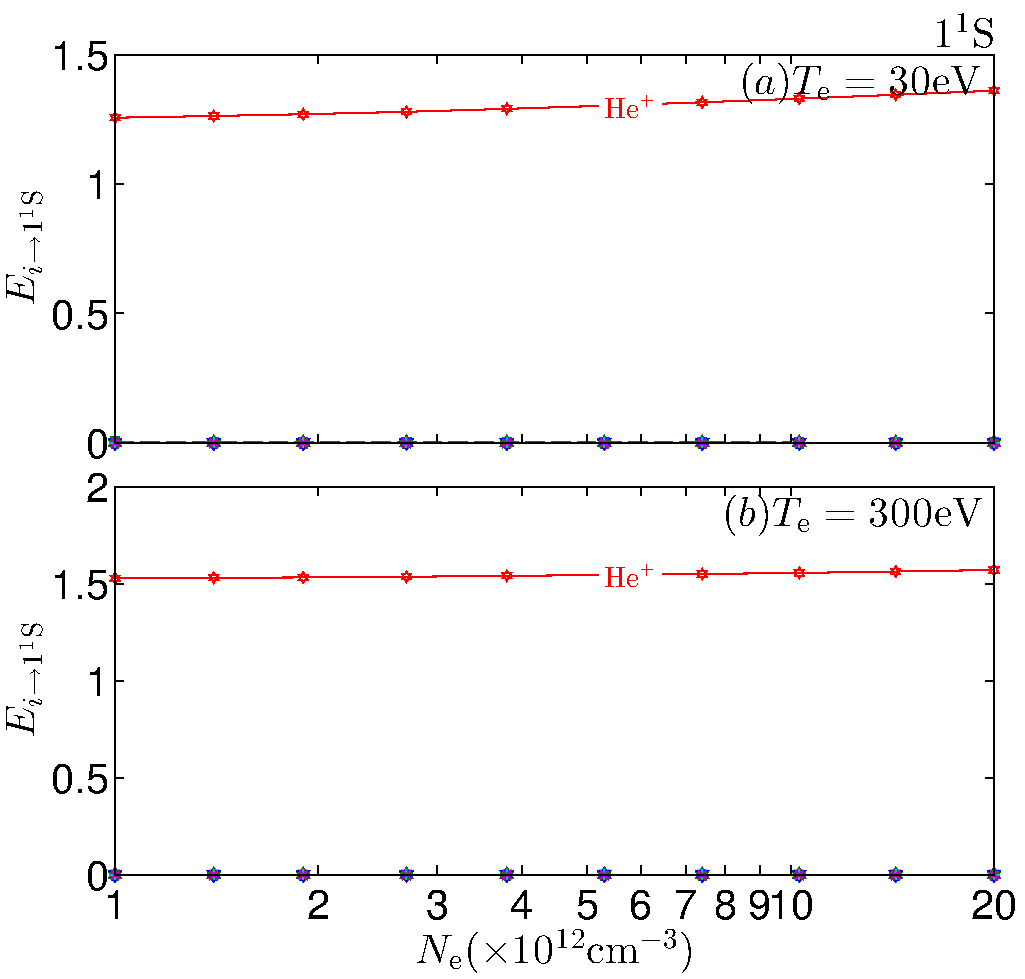
\includegraphics[width=0.6\textwidth]{11S-error-propagation-coefficient.pdf}
    \caption{所有能级至基态 $1^1{\rm S}$ 直接产生过程速率系数的不确定性传递函数}
    \label{fig:appendix:error-prop:1}
\end{figure}

\begin{figure}[H]
    \centering
    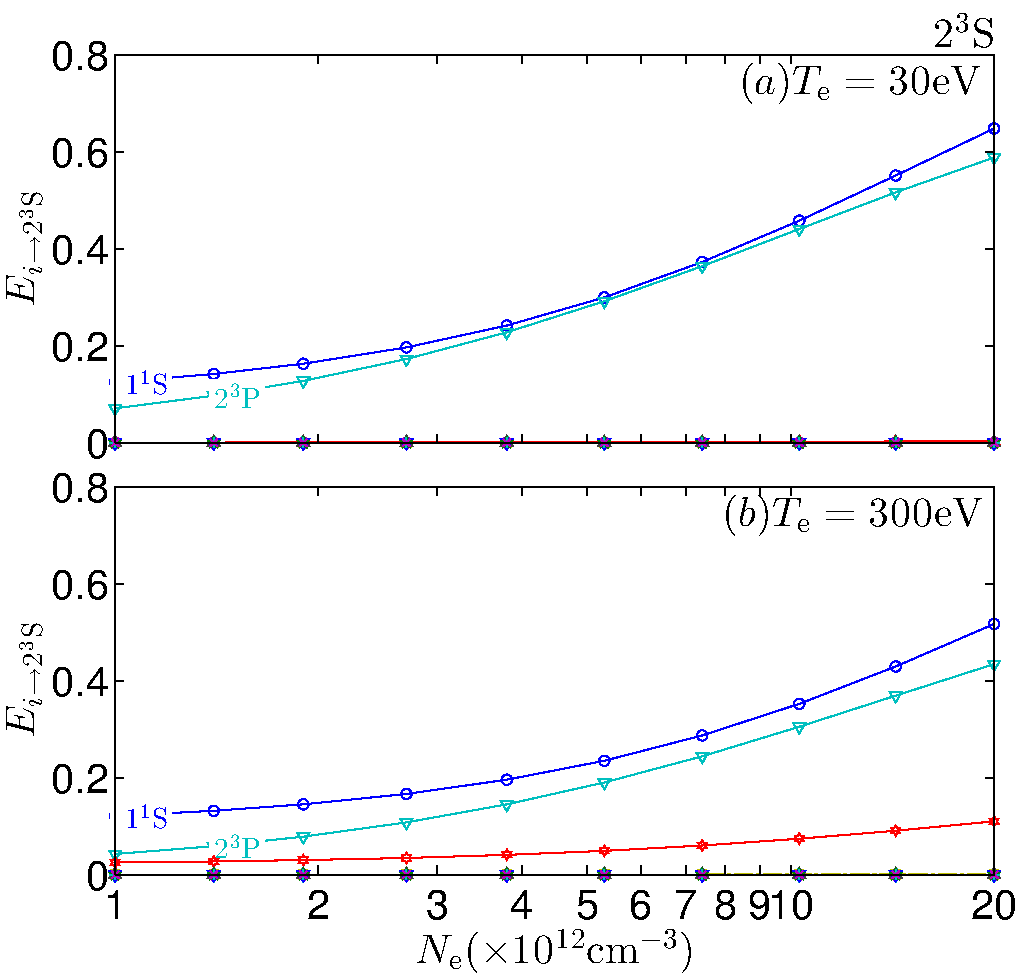
\includegraphics[width=0.6\textwidth]{23S-error-propagation-coefficient.pdf}
    \caption{所有能级至亚稳态 $2^3{\rm S}$ 直接产生过程速率系数的不确定性传递函数}
    \label{fig:appendix:error-prop:2}
\end{figure}

\begin{figure}[H]
    \centering
    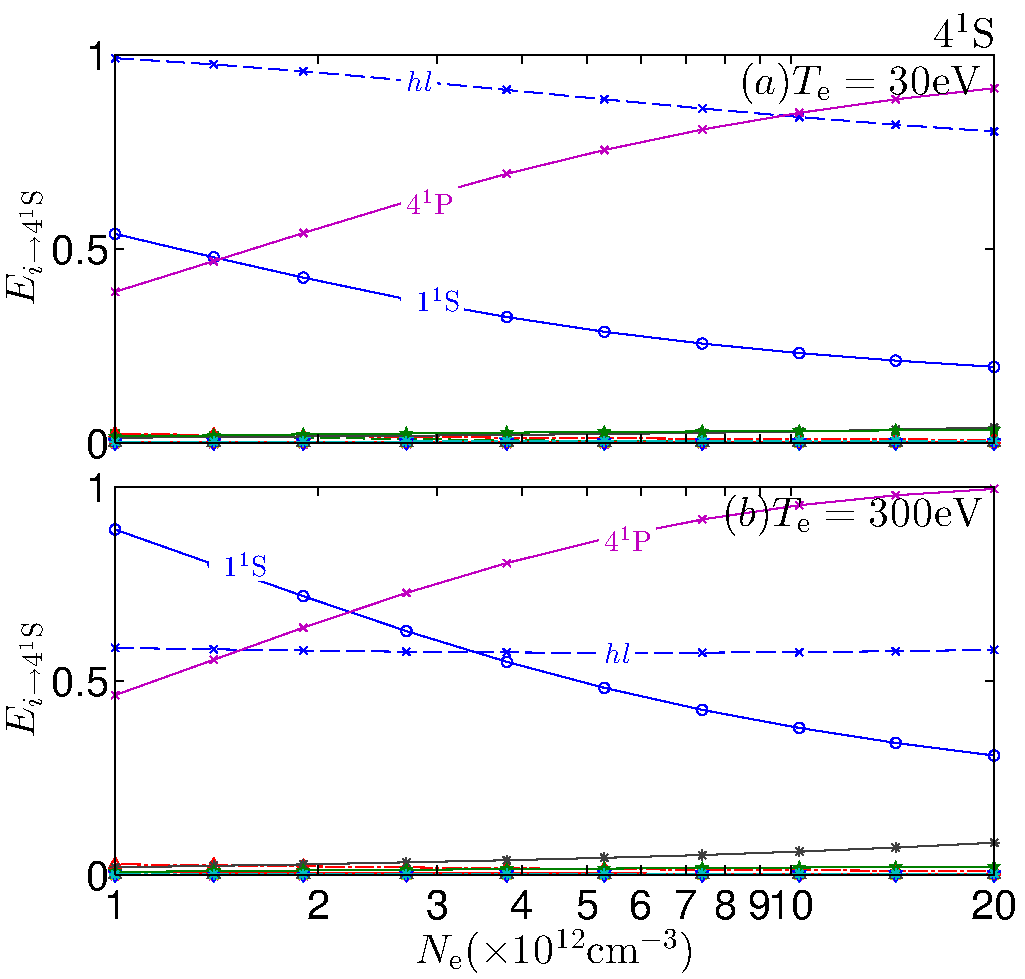
\includegraphics[width=0.6\textwidth]{41S-error-propagation-coefficient.pdf}
    \caption{所有能级至 $4^1{\rm S}$ 能级直接产生过程速率系数的不确定性传递函数}
    \label{fig:appendix:error-prop:3}
\end{figure}

\begin{figure}[H]
    \centering
    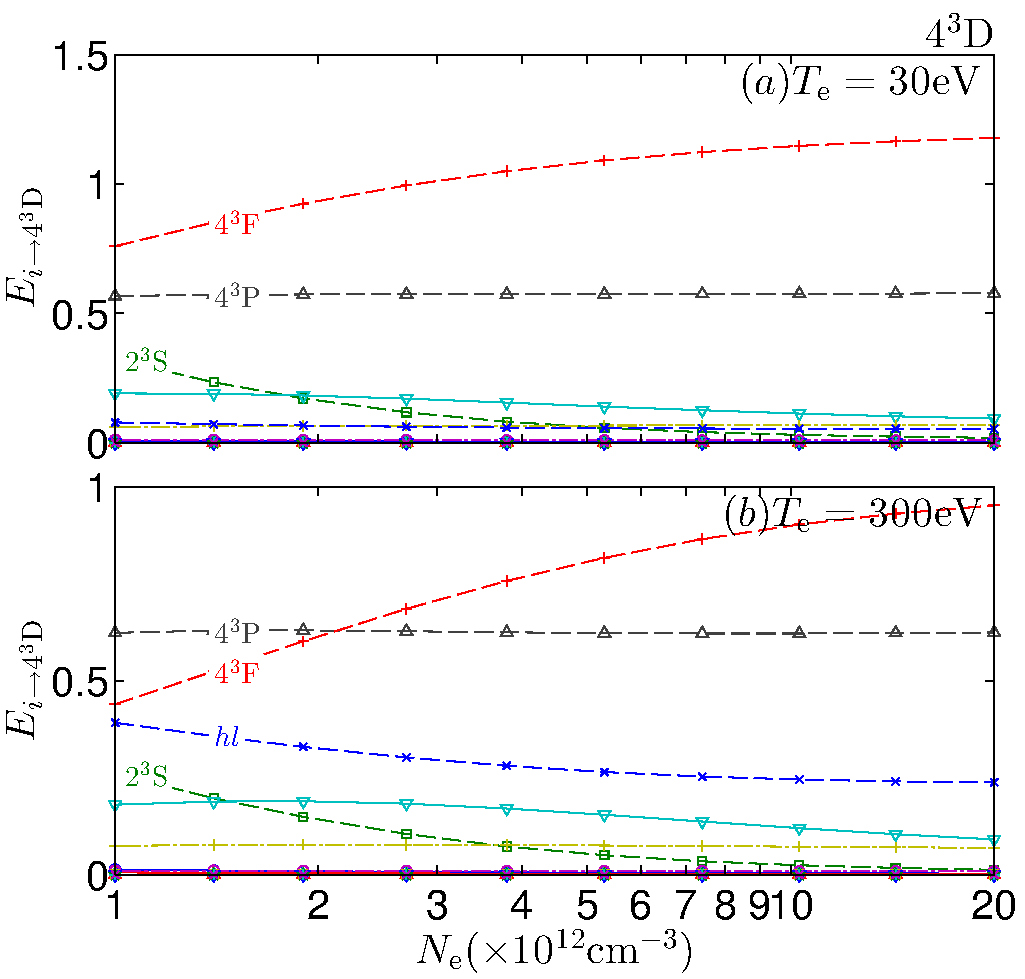
\includegraphics[width=0.6\textwidth]{43D-error-propagation-coefficient.pdf}
    \caption{所有能级至 $4^3{\rm D}$ 能级直接产生过程速率系数的不确定性传递函数}
    \label{fig:appendix:error-prop:4}
\end{figure}

\begin{figure}[H]
    \centering
    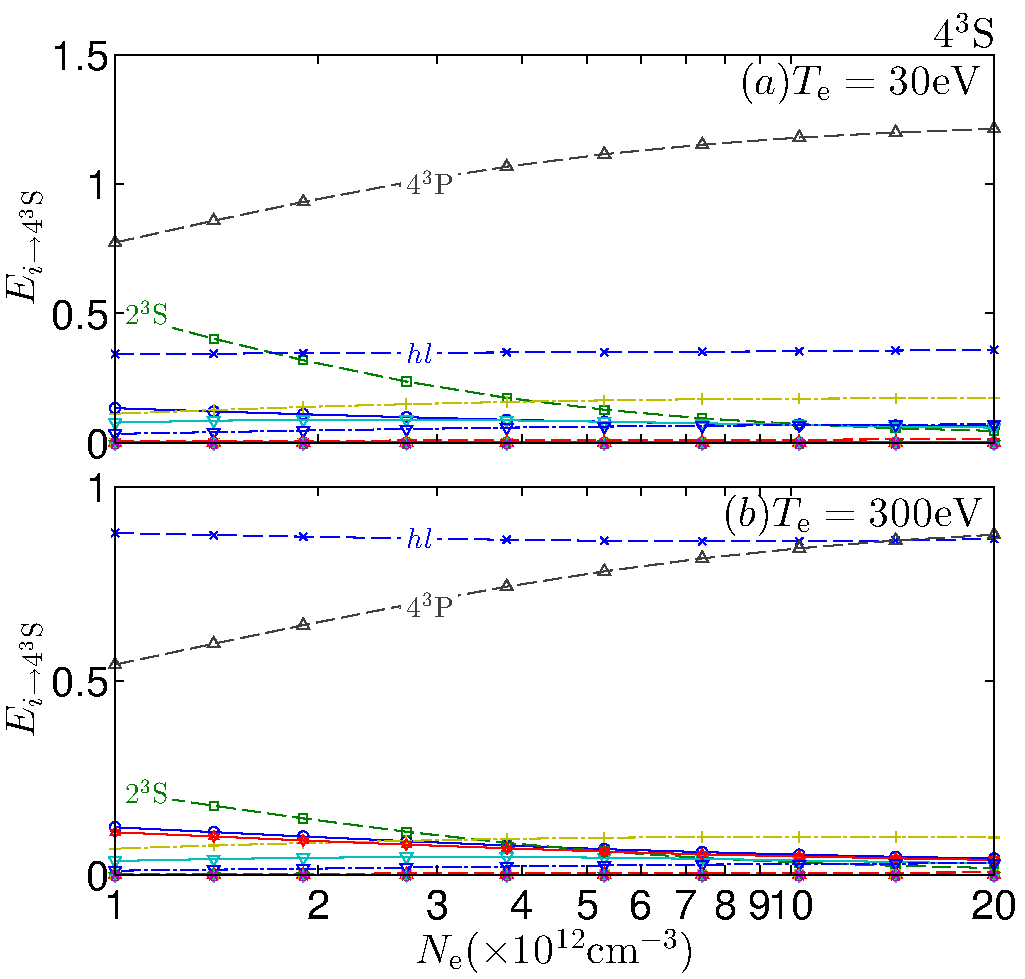
\includegraphics[width=0.6\textwidth]{43S-error-propagation-coefficient.pdf}
    \caption{所有能级至 $4^3{\rm S}$ 能级直接产生过程速率系数的不确定性传递函数}
    \label{fig:appendix:error-prop:5}
\end{figure}

\begin{figure}[H]
    \centering
    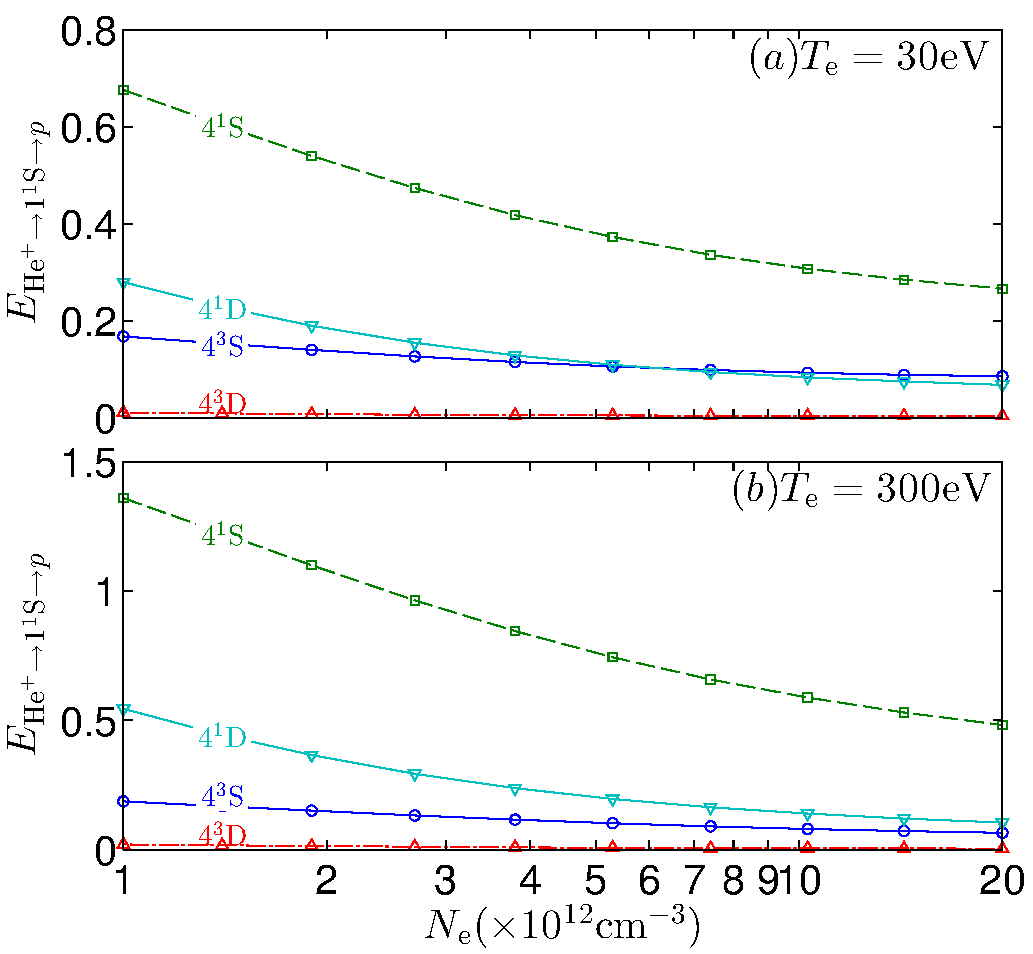
\includegraphics[width=0.6\textwidth]{HeII1p-error-propagation-coefficient.pdf}
    \caption{所有能级至 ${\rm He}^+$ 离子复合到基态能级 $1^1{\rm S}$ 的速率系数不确定性经二级反应过程至 $n=4$ 能级的传递函数}
    \label{fig:appendix:error-prop:6}
\end{figure}

\begin{figure}[H]
    \centering
    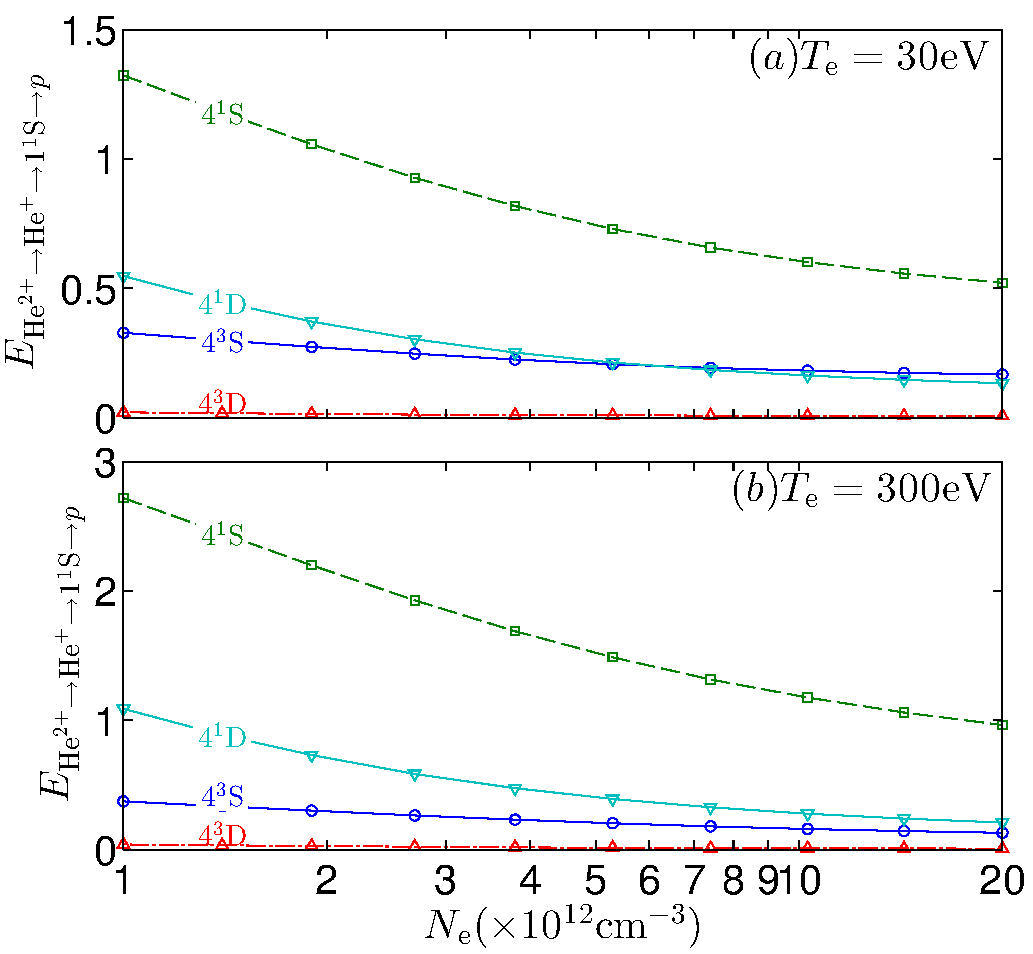
\includegraphics[width=0.6\textwidth]{HeIIIHeII1p-error-propagation-coefficient.pdf}
    \caption{${\rm He}^{2+}$ 离子复合到 ${\rm He}^+$ 的速率系数经三级级反应过程至 $n=4$ 能级的传递函数}
    \label{fig:appendix:error-prop:7}
\end{figure}

\begin{figure}[H]
    \centering
    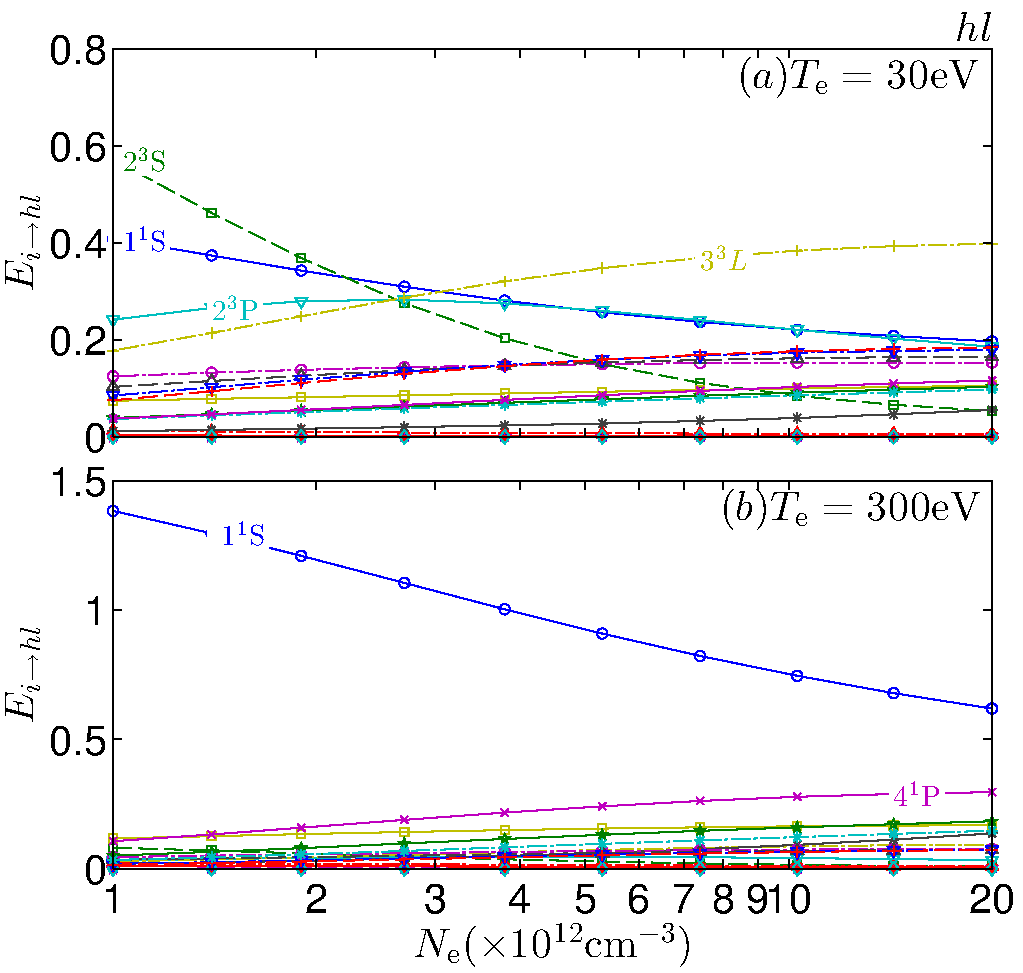
\includegraphics[width=0.6\textwidth]{hl-error-propagation-coefficient.pdf}
    \caption{其他能级至 $n\ge5$ 高能级 $hl$ 速率系数的传递函数}
    \label{fig:appendix:error-prop:8}
\end{figure}
